\documentclass{article}

\usepackage[margin=3cm]{geometry}

\usepackage{fancyhdr}
\pagestyle{fancy}
\usepackage{graphicx}
\usepackage{color}
\usepackage{xcolor}
\usepackage{hyperref}
\usepackage{cleveref}
\usepackage{tcolorbox}
%% Define no indent with line skip with new paragraph
\usepackage{parskip}

\definecolor{code}{rgb}{.92,.92,.99}
\definecolor{codered}{rgb}{.92,.62,.62}
\definecolor{darkgreen}{rgb}{.2,.62,.18}
\usepackage{listings}
\lstset{xrightmargin=10pt,xleftmargin=10pt,language=Java,captionpos=b,tabsize=3,frame=none,keywordstyle=\color{blue},commentstyle=\color{darkgreen},stringstyle=\color{red},showstringspaces=false,basicstyle=\footnotesize\ttfamily,emph={label},backgroundcolor=\color{code}}
%%numbers=left,numberstyle=\tiny,numbersep=5pt,breaklines=true,\

\usepackage{soul}
\lstdefinestyle{Bash}
{language=bash,
  escapechar=!,
  backgroundcolor=\color{white},
  columns=fullflexible,
  breaklines=true,         
  breakatwhitespace=false,
  inputencoding=utf8x,
  keywordstyle=\color{black},
  basicstyle=\small\ttfamily,
%  morekeywords={peter@kbpet},
%  alsoletter={:~$},
%  morekeywords=[2]{peter@kbpet:},
%  keywordstyle=[2]{\color{red}},
%  literate={\$}{{\textcolor{red}{\$}}}1 
%         {:}{{\textcolor{red}{:}}}1
%         {~}{{\textcolor{red}{\textasciitilde}}}1,
  literate={~}{\raisebox{-0.5ex}{\textasciitilde}}1,
}

\newenvironment{code}
{\begin{minipage}[l]{\textwidth}}
{\end{minipage}}

\newtcolorbox{mybox}{colback=blue!5!white,colframe=blue!75!black}

%\newcommand{\ccpmaketitle}[4][Roland Meertens, Christophe de Wagter, Guido de Croon, Tom van Dijk] {
%	\author{#1}
%	\title{\bf Crash Course Paparazzi 2020\\#2\\{\large #4#3}}
%	\date{February 2020}
%	\setlength{\parindent}{0em}
%	\maketitle
%}
\def\coursebranch{mavlabCourse\the\year}

% Set headers and footers
\fancyhead[LO,LE]{Crash Course Paparazzi \the\year}
\renewcommand{\chaptermark}[1]{\markboth{\chaptername\ \thechapter.\ #1}{}}
\fancyfoot[LO,LE]{{\small Crash Course Paparazzi \the\year}}
\fancyfoot[CO,CE]{\thepage}


\begin{document}
\ccpmaketitle{Computer vision}{\ldots Making your drone see something}{lesson 4}

\subsection*{Introduction}
Welcome to the most important part of this course: understanding how vision works. When using image processing right your drone can perform the most awesome tricks. However: when you do it wrong your drone will crash. 

\subsection*{Goals of this exercise}
\begin{itemize}
\item Finding the camera data
\item The format of the image
\item Your first project
\end{itemize}

\subsection*{Finding the camera data}
To get data out of the front facing camera in paparazzi you have to include the video\_thread.xml module in your airframe file, and define VIDEO\_THREAD\_CAMERA to front\_camera. After you added this you can create a new module that does something with the data of the front camera. A nice example for such a module is the colorfilter module.

If you want to see what the image looks like on your computer after it comes out of the camera or the color filter you have to can also include the video\_rtp\_stream  module. 
The modules part of your airframe file might now look like this:
\begin{verbatim}
  <firmware name="rotorcraft">
    ...
    <!-- Video/Camera modules -->
    <module name="video_thread" />
    <module name="cv_colorfilter">
      <define name="COLORFILTER_CAMERA" value="front_camera" />
    </module>
    <module name="orange_avoider" />
    <module name="video_rtp_stream">
      <define name="VIEWVIDEO_CAMERA" value="front_camera" />
      <define name="VIEWVIDEO_FPS" value="10"/>
      <define name="VIEWVIDEO_STREAM_VIDEO" value="TRUE" />
      <define name="VIEWVIDEO_DOWNSIZE_FACTOR" value="1" />
      
      <define name="VIEWVIDEO_SHOT_PATH" value="/data/ftp/internal_000" />
    </module>
  </firmware>
\end{verbatim}
Upload this to your bebop.

Start VLC and open \verb|conf/video.sdp| to view the video from the drone.
The Bebop's camera is rotated by 90 degrees. You can correct this in VLC by going to `Tools $\rightarrow$ Effects and filters $\rightarrow$ Video Effects $\rightarrow$ Geometry', checking `Transform' and selecting `Rotate by 270 degrees' below it.
 
If you open your ground control station and go to settings--ColorFilter you can change what is filtered by the colorfilter. Look at the YUV colorspace on Wikipedia (\url{https://en.wikipedia.org/wiki/YUV}) and try to find settings that filter the color orange. If you open the RTP stream you can see what pixels are selected, they become red. 

In the lab we tried filtering the color red, as found on our hands and little red and green balls. We used the following values, and obtained the following result:
\begin{verbatim}
y_min = 4
y_max = 91
u_min = 0
u_max = 124
v_min = 127
v_max = 255
\end{verbatim}

\begin{center}
\centering
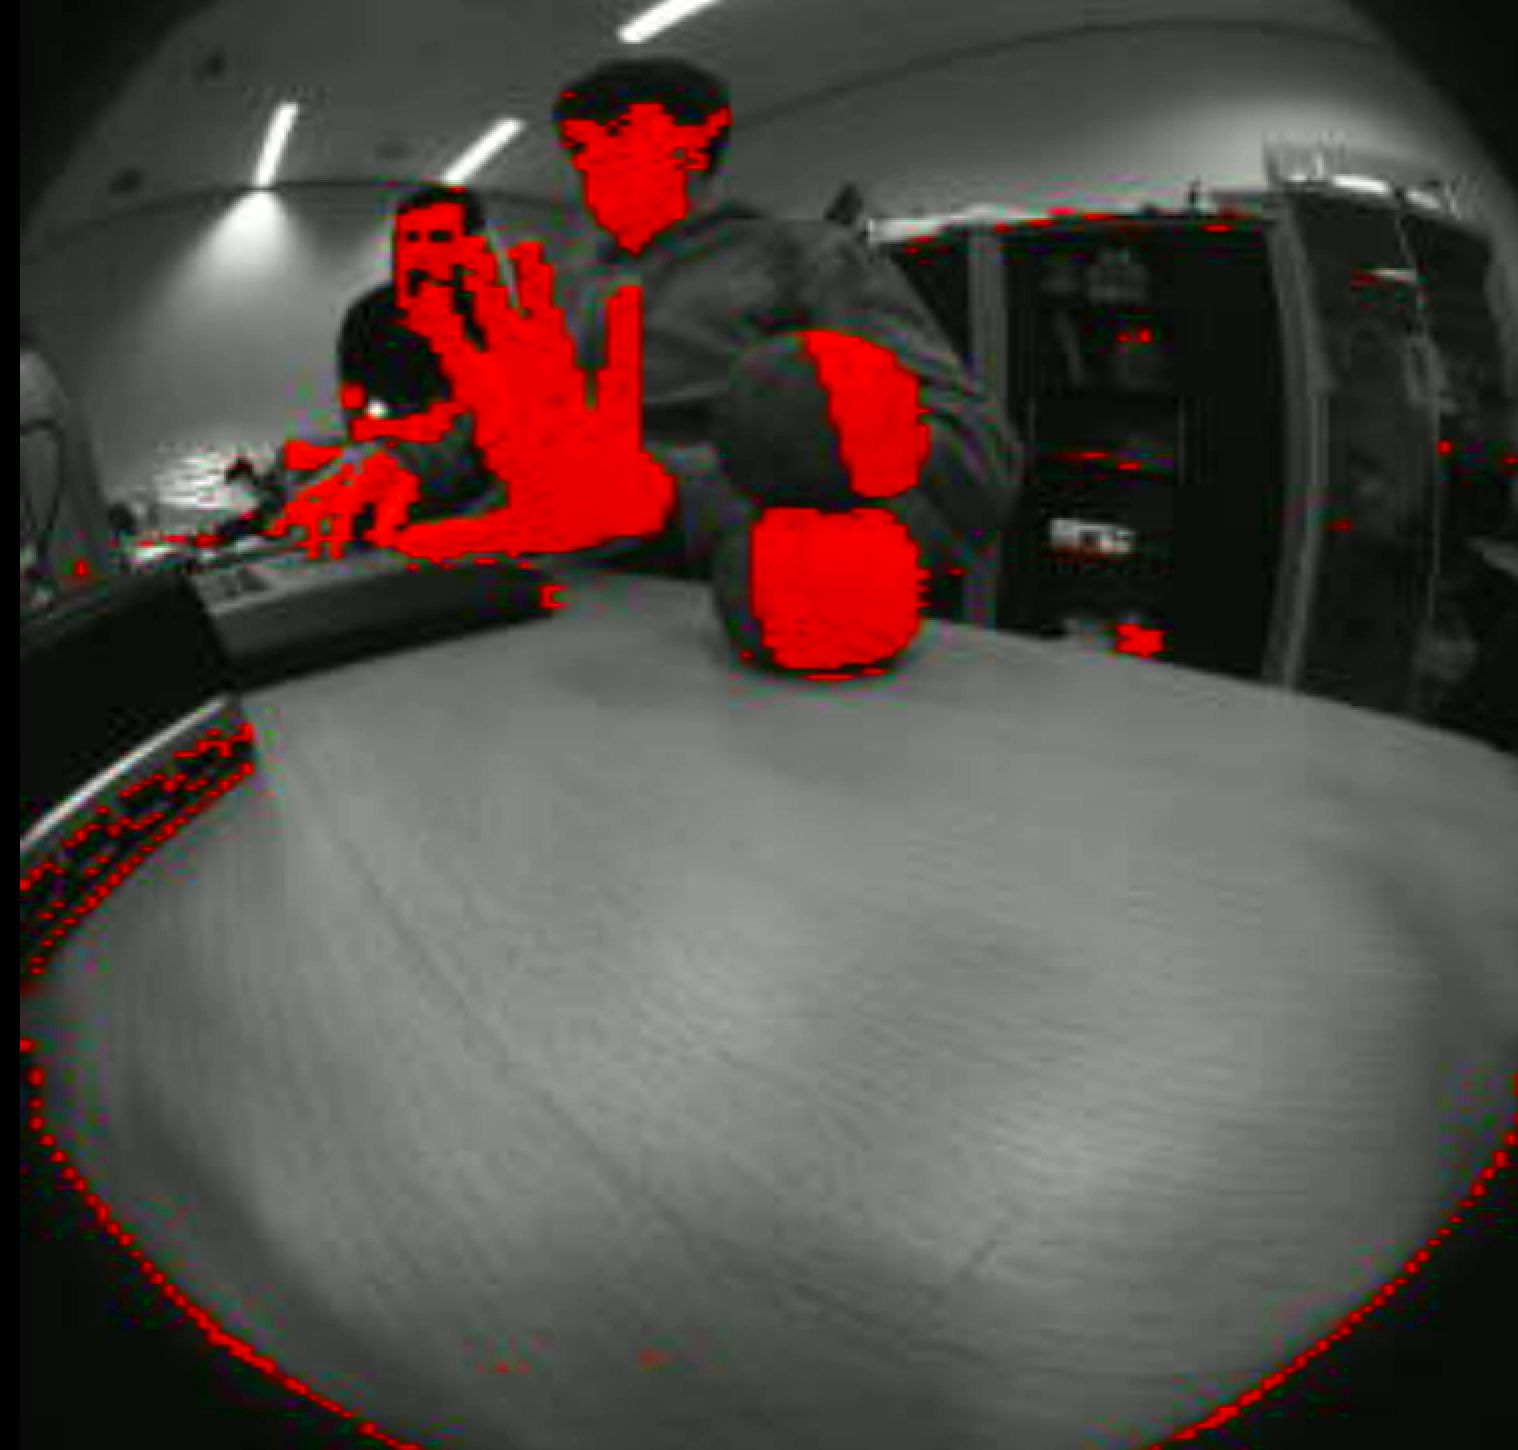
\includegraphics[width=0.75\linewidth]{filtered}
\end{center}

Note that streaming images takes a large amount of bandwith. This could cause your joystick of optitrack position commands to be delayed (causing instability) or not even arrive.

Take some time to check what the colorfilter does in the file colorfilter.c. 

In the colorfilter\_init function the function cv\_add\_to\_device is called with as argument the colorfilter\_func function and the front camera:
\begin{verbatim}

void colorfilter_init(void) {
  listener = cv_add_to_device(&COLORFILTER_CAMERA, colorfilter_func);
}

\end{verbatim}

Now each time the video thread gets an image from the camera it calls the colorfilter\_func function with the new image as an argument:

\begin{verbatim}
bool_t colorfilter_func(struct image_t* img) {
  // Filter
  color_count = image_yuv422_colorfilt(img,img,
      color_lum_min,color_lum_max,
      color_cb_min,color_cb_max,
      color_cr_min,color_cr_max
      );
  return FALSE;
}
\end{verbatim}
\begin{center}
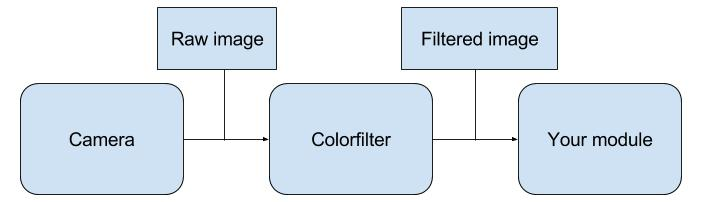
\includegraphics[width=0.8\linewidth]{camerafilter}
\end{center}

Note that the order in which you call cv\_add is important. The first function to get the image might edit the image. If you add modules that do something with the image, the first module you added in your airframe file will get the image first. The reason that the image might be changed is because the functions is passed a pointer to the image. 

The argument the function gets is a pointer to an image it is possible for a module to change the actual image. If you take a look at the colorfilter function you see this module does this. Colorfilter sets UV to zero (makes the unfiltered image grayscale) and enhances the color at the filtered colors. A second module added after the colorfilter will see a gray image with some enhanced colours. 

\subsection*{The format of the image}
The image you receive is yuv422, or UYVY. Per two pixels four bytes of data are recorded. The U and V together define the color and both pixels get the same color (but different intensity). Image.c has several functions that can be used with this format. Please take a look at this file and try to understand what these functions are doing, how you can use them, and what other functions would be useful. 

\subsection*{Your first project}
Now it is time to choose an exercise to learn how to program in Paparazzi using your flightplan skills, code skills and computer vision skills. The two options are:

\subsubsection*{Choice 1: Read a sign}
Fly to a position in the center of the arena. If you see a blue sign fly to a waypoint to the left, hover here for five seconds and go back to the center. If you see a red sign perform the same behaviour but fly to the right. 

\subsubsection*{Choice 2: Follow me!}
Create a real "selfie-drone" in which the drone follows an orange blob at a certain distance.

Start by hovering at a waypoint and determining where the orange blob is (more to the left or more to the right?) and adjust your heading based on this.

To start following you, you can determine the size of the blob. Is it too big? Fall back! Otherwise: fly forwards by slowly moving your waypoint.
\end{document}
